\documentclass[12pt]{article}

\usepackage{fullpage,parskip,csquotes,graphicx}
\usepackage{newpxtext,newpxmath}
\usepackage{setspace}
\setstretch{1.3}

% Fix {sub}section numbering to match Quarto output
\makeatletter
\renewcommand\thesubsection{\@arabic\c@subsection}
\makeatother

\usepackage[dvipsnames]{xcolor}
\usepackage{hyperref}
\hypersetup{
    colorlinks,
    linkcolor={red!50!black},
    citecolor={blue!60!black},
    urlcolor={blue!80!black}
}
\usepackage{cleveref}


\begin{document}

\title{Cryptography challenge: facilitator notes}
\author{The Alan Turing Institute}
\date{Last updated: \today}
\maketitle

\subsection*{General comments}

Timings, etc.

Whom to ask if you need help.

\subsection{Introduction}

For any students who are struggling to crack the initial cipher, the best place to start is the first and last lines, which are respectively ``Hello Bob'' and ``Alice''.
Hints to this include the capitalisation of the names, as well as the repeated letters in Bob's name.
With these letters filled in, the rest of the message becomes

\begin{displayquote}
Hello Bob,

Ho* a*e *o*?\\
Le*'* *ee* o* *o**a*!

Alice
\end{displayquote}

(The answer is Monday.)

\pagebreak
\section*{Symmetric ciphers}

\subsection{Caesar cipher}

The Caesar cipher page did not seem to pose any problems in the 2023 sessions.
The answer for the question at the bottom is \texttt{HIDDENMESSAGE}.

For very advanced students, you may wish to ask them why there are only 26 possibilities (or 25 useful ones) for a Caesar cipher.
The answer is that there are only 26 letters in the English alphabet, so shifting by 27 is the same as shifting by 1---this is a very early example of the modular arithmetic which will be covered in the second half.

\subsection{Monoalphabetic ciphers}

For why texts may deviate from the standard frequency distribution: a simple one is the use of different spellings, e.g. American vs British English. More examples can be found at \url{https://en.wikipedia.org/wiki/Letter_frequency}.

One thing worth pointing out is that frequencies are only really stable if the text is long enough.

The decoding challenge is probably the part of the first half that students will spend the most time on, if only because there is a lot of trial-and-error involved.
It is generally obvious that the most common letter in English is E, but the next most common letters tend to depend on the text from which it is drawn, so are less immediately useful.

From the frequency analysis, students should be able to guess that ciphertext \texttt{I} corresponds to plaintext \texttt{E}.
Furthermore, in the ciphertext, the trigram \texttt{PVI} appears regularly.
Together this implies that \texttt{P} corresponds to \texttt{T} and \texttt{V} corresponds to \texttt{H}.
Sensible next steps would be to try to match up the remaining common letters, namely \texttt{Y} and \texttt{A}: these correspond to \texttt{A} and \texttt{O} in plaintext respectively.

The full answers are:

\begin{center}
    \ttfamily
    \begin{tabular}{rccccccccccccc}
        \textrm{ciphertext} & A & B & C & D & E & F & G & H & I & J & K & L & M \\
        \textrm{plaintext}  & O & B & S & G & P & I & M & C & E & F & Q & K & V \\
        \hline
        \textrm{ciphertext} & N & O & P & Q & R & S & T & U & V & W & X & Y & Z \\
        \textrm{plaintext}  & X & R & T & W & N & Z & D & L & H & J & Y & A & U \\
    \end{tabular}
\end{center}

\subsection{Vigen{\`e}re cipher}

Reading the Vigen{\`e}re square the other way around works because the square is symmetric: at a more fundamental level this is because the encoding is effectively carried out by adding two numbers, and addition is a commutative operation.

We found that providing a concrete example of calculating the IoC for a short piece of text was helpful for aiding students' understanding.

To prove that the IoC for long, random text is 1: let the length of the text be $N$.
Then, we have that $n_\text{A} = n_\text{B} = \cdots = N/26$, and so:

$$\text{IoC} = 26 \cdot \frac{N/26(N/26 - 1) \cdot 26}{N(N - 1)} = \frac{N - 26}{N - 1},$$

and as $N \to \infty$, this tends to 1. (Strictly, we only need that $N \gg 26$ or that $N / 26 \gg 1$, which the question states.)

For the decoding challenge, the key is (quite literally) \texttt{KEY}.
The text is the opening of Turing's 1936 paper \emph{On Computable Numbers, with an Application to the Entscheidungsproblem} (DOI: \href{https://doi.org/10.1112/plms/s2-42.1.230}{\texttt{10.1112/plms/s2-42.1.230}}).

\subsection{Enigma}

\pagebreak
\section*{Asymmetric ciphers}

\subsection{Modular arithmetic I}

Generally, it really helps if you can use pen-and-paper diagrams to illustrate the idea of the `remainder'.
For example, this is a pictorial argument for $(a + b) \equiv (p + q) \bmod n$:

\begin{center}
    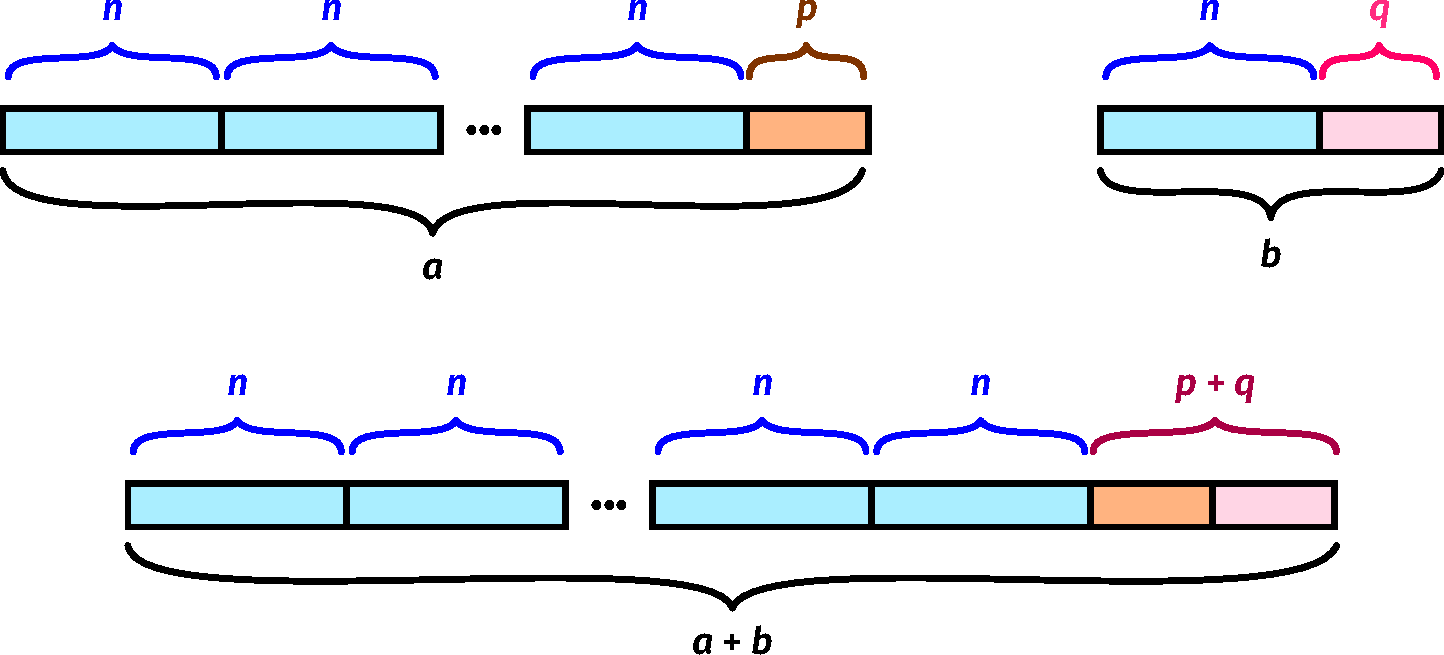
\includegraphics[width=0.8\textwidth]{modulo.pdf}
\end{center}

Mathematically, the proof for $(ab) \equiv (pq) \bmod n$ follows the same structure as for the earlier one.
Let $a = p + cn$, and $b = q + dn$. Then
\begin{align*}
    ab &= (p + cn)(q + dn) \\
       &= pq + (pd + qc)n + cdn^2 \\
       &\equiv pq \bmod n.
\end{align*}

One thing that students are very tempted to do is to `factorise out' the ${} \bmod n$ part, like this:
\begin{align*}
    a + b \equiv (p \bmod n) + (q \bmod n) = (p + q) \bmod n.
\end{align*}

This is not valid, because the $\bmod$ operator is not a function, and so does not distribute over addition.
To explain this, you could use the example of subtraction: say $a = p - x$ and $b = q - x$.
You certainly cannot `factorise out' the ${}-x$ part like this:
\begin{equation*}
a + b = (p - x) + (q - x) = (p + q) - x.
\end{equation*}

The proof by induction goes as follows:

\begin{itemize}
    \item \textit{Base case.} Consider $m = 1$. Then $a^1 \equiv a \equiv p \equiv p^1 \bmod n$.
    \item \textit{Inductive step.} Assume that $(a^m) \equiv (p^m) \bmod n$ for some $m$. Then
        \begin{align*}
            a^{m+1} = a^m \cdot a \equiv p^m \cdot p \bmod n = p^{m+1} \bmod n,
        \end{align*}
        where the middle equality follows from statement (2).
\end{itemize}

For the challenge question, the answer is $7^{175} \bmod 16 = 7$.
The suggestion to find a pattern should lead students to notice that
\begin{align*}
    7^1 \bmod 16 &= 7 \\
    7^2 \bmod 16 &= 1 \\
    7^3 \bmod 16 &= 7
\end{align*}
and so on, which implies that any odd power of 7 is congruent to 7 modulo 16.

Formally, we can show this by noting that $7^2 = 49 \equiv 1 \bmod 16$. So,
\begin{align*}
    7^{175} \bmod 16 &= (7^{173} \cdot 7^2) \bmod 16 \\
                     &\equiv (7^{173} \cdot 1) \bmod 16 \quad \text{(using statement (2) in the notes)} \\
                     &= 7^{173} \bmod 16 \\
                     &\equiv (7^{171} \cdot 7^2) \bmod 16 \\
                     &\quad\vdots \\
                     &\equiv 7^1 \bmod 16 = 7.\\
\end{align*}

\subsection{RSA scheme I}

\subsection{Modular arithmetic II}

The answer for the exercise at the bottom of the page is $d = 325$.

Specifically: we need $ed + y\phi = 1$, or substituting in the values, $13d + 352y = 1$.

If we divide $352$ by $13$ we find that $352 = (13 \cdot 27) + 1$, or equivalently, $(13 \cdot -27) + (352 \cdot 1) = 1$.
This suggests a value of $d = -27$ and $y = 1$.
As before, we need to add and subtract $(13 \cdot 352)$ to make $d$ positive:
\begin{align*}
    1 &= (13 \cdot -27) & &+ (352 \cdot 1) \\
      &= (13 \cdot -27) + (13 \cdot 352) & &- (13 \cdot 352) + (352 \cdot 1) \\
      &= (13 \cdot (-27 + 352)) & &+ (352 \cdot (1 - 13)) \\
      &= (13 \cdot 325) & &+ (352 \cdot (-12)) \\
      &= (13d) & &+ (352y),
\end{align*}
which lets us read off $d = 325$ (and the unneeded $y = -12$).

\subsection{RSA scheme II}

To crack the RSA scheme, we need to find $d$ (using the Euclidean algorithm), which requires us to know the value of $\phi$.
Because $\phi = (p - 1)(q - 1)$, this in turn means that we need to know the prime factors $p$ and $q$ which are multiplied together to form $n$.

In the first case where $n$ is small (143), this is trivial: we have that $p = 11$ and $q = 13$.
Thus $\phi = 10 \cdot 12 = 120$, and we can find $d = 103$ using exactly the same steps as on the previous page.
Plugging this value of $d$ into the script gives the correct answer $m = 50$.

In the second case, factorising $373577$ is much harder (and so is calculating $d$, at least without a computer).
The answer is $m = 500$, but the students are \textit{not} expected to complete this.

For the final section involving the logarithmic graph, the exact value of $n$ found will vary on the computer (and browser) being used.
On one occasion, Chrome outperformed Safari by a factor of 3.
In any case, when tested on Firefox 119.0 on a 2021 MacBook Pro (32 GB RAM, Apple M1 Pro), the regression equation obtained was
$$\log_{10} (t / \text{ms}) = 0.43\log_{10}{n} - 4.00$$
and plugging in a time $t = 365 \cdot 24 \cdot 60 \cdot 60 \cdot 1000~\text{ms}$ (approximately 1 year) gives $\log_{10}n = 33.72$, i.e., somewhere around $5 \cdot 10^{33}$.

It should be noted that the prime factorisation algorithm used is hardly the most performant (it is a brute-force search).
However, it is perfectly serviceable in illustrating the point that the RSA scheme requires large numbers.

\pagebreak

\subsection{Cryptography Game Resources}

\end{document}
